\section{Introducción}

\subsection{FuDePAN}
	\begin{frame}{\textbf{FuDePAN}}
  	  \par La \textbf{Fu}ndación para el \textbf{De}sarrollo de la \textbf{P}rogramación en \textbf{Á}cidos \textbf{N}ucleicos es una ONG (organización no gubernamental) concebida	para fomentar el desarrollo de técnicas y tecnologías para la Programación en Ácidos Nucleicos, al servicio de la salud humana.\\[0.2cm]

	  \pause
  	  \begin{itemize}
      	\item Fundada en 2006.
      	\item Bioinformática ingenieril.
      	\item I+D.
      	\item Colaboran
      	  \begin{itemize}
      	      \item Estudiantes: Voluntarios y tesistas
      	      \item Profesionales: Ámbito industrial y académico.
      	  \end{itemize}
      	\item Todo lo desarrollado por la fundación se encuentra bajo GPLv3.
      \end{itemize}	
	\end{frame}

    \begin{frame}{\textbf{FuDePAN (cont.)}}
       \large{\textbf{Pilares}}
       \begin{center}
           
\includegraphics[scale=0.30]{images/fudesuma.png}
       \end{center}
       \pause
       \begin{block}{Naturaleza de los problemas}
           \begin{itemize}
               \item Corren mucho tiempo
               \item Alta performance
               \item Resultados impactan en nuevos problemas y personas.
           \end{itemize}
      \end{block}
	\end{frame}

\subsection{Motivación}
  \begin{frame}\frametitle{\textbf{Motivación}}      
    \begin{itemize}
      \item \textbf{Dado a que:}
        FuDePAN tenía un trabajo disponible.
      \item \textbf{Surgió la necesidad de:}
        Investigar y desarrollar un software.
      \item \textbf{Objetivo Principal:}
        contrastar una teoría (una hipótesis).
    \end{itemize}

    \begin{minipage}{3cm \textwidth}
       \begin{block}{\small{Dr. Daniel Rabinovich}}
        \hspace*{.25cm}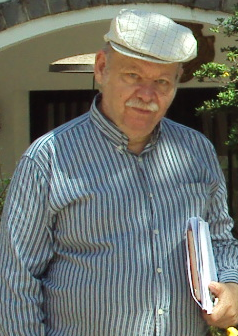
\includegraphics[scale=.25]{images/danielR.png}        
        \vskip .1cm
        \hspace*{.9cm}
\includegraphics[scale=.25]{images/inbird.jpg}
      \end{block}      
    \end{minipage}
    \begin{minipage}{6cm}
      \begin{center}
        \pause
        \textbf{Perspectiva Personal}
        \begin{itemize}
          \item Tarea desafiante.
          \item Integrarse en un grupo de desarrollo formado.
          \item Adaptarse a nuevos entornos.
          \item Contribuir a la salud.
          \item Retribuir con trabajo.
        \end{itemize}
      \end{center}
    \end{minipage}       
    
  \end{frame}